\documentclass[journal]{IEEEtran}
\usepackage[a5paper, margin=10mm]{geometry}
%\usepackage{lmodern} % Ensure lmodern is loaded for pdflatex
\usepackage{tfrupee} % Include tfrupee package


\setlength{\headheight}{1cm} % Set the height of the header box
\setlength{\headsep}{0mm}     % Set the distance between the header box and the top of the text


%\usepackage[a5paper, top=10mm, bottom=10mm, left=10mm, right=10mm]{geometry}

%
\setlength{\intextsep}{10pt} % Space between text and floats

\makeindex


\usepackage{cite}
\usepackage{amsmath,amssymb,amsfonts,amsthm}
\usepackage{algorithmic}
\usepackage{graphicx}
\usepackage{textcomp}
\usepackage{xcolor}
\usepackage{txfonts}
\usepackage{listings}
\usepackage{enumitem}
\usepackage{mathtools}
\usepackage{gensymb}
\usepackage{comment}
\usepackage[breaklinks=true]{hyperref}
\usepackage{tkz-euclide} 
\usepackage{listings}
\usepackage{multicol}
\usepackage{xparse}
\usepackage{gvv}
%\def\inputGnumericTable{}                                 
\usepackage[latin1]{inputenc}                                
\usepackage{color}                                            
\usepackage{array}                                            
\usepackage{longtable}                                       
\usepackage{calc}                                             
\usepackage{multirow}                                         
\usepackage{hhline}                                           
\usepackage{ifthen}                                               
\usepackage{lscape}
\usepackage{tabularx}
\usepackage{array}
\usepackage{float}
\usepackage{ar}
\usepackage[version=4]{mhchem}


\newtheorem{theorem}{Theorem}[section]
\newtheorem{problem}{Problem}
\newtheorem{proposition}{Proposition}[section]
\newtheorem{lemma}{Lemma}[section]
\newtheorem{corollary}[theorem]{Corollary}
\newtheorem{example}{Example}[section]
\newtheorem{definition}[problem]{Definition}
\newcommand{\BEQA}{\begin{eqnarray}}
\newcommand{\EEQA}{\end{eqnarray}}

\theoremstyle{remark}


\begin{document}
\bibliographystyle{IEEEtran}
\onecolumn

\title{4.11.5}
\author{INDHIRESH S- EE25BTECH11027}
\maketitle


\renewcommand{\thefigure}{\theenumi}
\renewcommand{\thetable}{\theenumi}

\textbf{Question}. Find the equation of the plane passing through the points $(2, 5, -3)$, $(-2, -3, 5)$, and $(5, 3, -3)$. Also, find the point of intersection of this plane with the line passing through points $(3, 1, 5)$ and $(-1, -3, -1)$.\\
\textbf{Solution}:\\
Let us solve the given equation theoretically and then verify the solution computationally. \\
Let the given points be:
\begin{align}
   \Vec{A}=\myvec{2\\5\\-3}\;,\Vec{B}=\myvec{-2\\-3\\5}\;and\;\Vec{C}=\myvec{5\\3\\-3}
\end{align}
For equation of plane:

\begin{align}
   \myvec{\Vec{A}&\Vec{B}&\Vec{C}}^T\Vec{n}=\myvec{1\\1\\1}
\end{align}

\begin{align}
   \myvec{2&-2&5\\5&-3&3\\-3&5&-3}^T\Vec{n}=\myvec{1\\1\\1}
\end{align}

\begin{align}
   \myvec{2 & 5 & -3\\-2 & -3 & 5\\5 & 3 & -3}\Vec{n}=\myvec{1\\1\\1} \Rightarrow \augvec{3}{1}{2 & 5 & -3&1\\-2 & -3 & 5&1\\5 & 3& -3&1}
\end{align}

\begin{align}
   \augvec{3}{1}{2 & 5 & -3&1\\-2 & -3 & 5&1\\5 & 3& -3&1}\xleftrightarrow[R_2\longleftarrow R_2+R_1]{R_3\longleftarrow R_3-\frac{5}{2}R_1}  \augvec{3}{1}{2 & 5 & -3&1\\0 & 2 & 2&2\\0 & \frac{-19}{2}& \frac{9}{2}&\frac{-3}{2}}
\end{align}

\begin{align}
     \augvec{3}{1}{2 & 5 & -3&1\\0 & 2 & 2&2\\0 & \frac{-19}{2}& \frac{9}{2}&\frac{-3}{2}} \xleftrightarrow{R_2\longleftarrow\frac{1}{2}R_2} \augvec{3}{1}{2 & 5 & -3&1\\0 & 1 & 1&1\\0 & \frac{-19}{2}& \frac{9}{2}&\frac{-3}{2}}
\end{align}

\begin{align}
   \augvec{3}{1}{2 & 5 & -3&1\\0 & 1 & 1&1\\0 & \frac{-19}{2}& \frac{9}{2}&\frac{-3}{2}} \xleftrightarrow{R_3\longleftarrow R_3+\frac{19}{2}R_2} \augvec{3}{1}{2 & 5 & -3&1\\0 & 1 & 1&1\\0 & 0& 14&8}
\end{align}
\begin{align}
     \augvec{3}{1}{2 & 5 & -3&1\\0 & 1 & 1&1\\0 & 0& 14&8} \xleftrightarrow{R_3\longleftarrow\frac{R_3}{14}}\augvec{3}{1}{2 & 5 & -3&1\\0 & 1 & 1&1\\0 & 0& 1&\frac{4}{7}}
\end{align}
\begin{align}
    \augvec{3}{1}{2 & 5 & -3&1\\0 & 1 & 1&1\\0 & 0& 1&\frac{4}{7}}\xleftrightarrow[R_2\longleftarrow R_2-R_3]{R_1\longleftarrow R_1+3R_3} \augvec{3}{1}{2 & 5 & 0&\frac{19}{7}\\0 & 1 &0 &\frac{3}{7}\\0 & 0& 1&\frac{4}{7}}
\end{align}
\begin{align}
    \augvec{3}{1}{2 & 5 & 0&\frac{19}{7}\\0 & 1 &0 &\frac{3}{7}\\0 & 0& 1&\frac{4}{7}}\xleftrightarrow{R_1\longleftarrow R_1-5R_2}  \augvec{3}{1}{2 & 0 & 0&\frac{4}{7}\\0 & 1 &0 &\frac{3}{7}\\0 & 0& 1&\frac{4}{7}}
\end{align}
\begin{align}
     \augvec{3}{1}{2 & 0 & 0&\frac{4}{7}\\0 & 1 &0 &\frac{3}{7}\\0 & 0& 1&\frac{4}{7}}\xleftrightarrow{R_1\longleftarrow \frac{R_1}{2}}\augvec{3}{1}{1 & 0 & 0&\frac{2}{7}\\0 & 1 &0 &\frac{3}{7}\\0 & 0& 1&\frac{4}{7}}
\end{align}

The equation of plane can be given as:

\begin{align}
\Vec{n}^T\Vec{x}=c
  \end{align}
Therefore the equation of plane can be given as:
\begin{align}
  \myvec{2\\3\\4}^T\Vec{x}=7
\end{align}
Where
\begin{align}
    n=\myvec{2\\3\\4}\;\;and\;\; c=7
\end{align}
The equation of line passing through the points $(3,1,5)$ and $(-1,-3,-1)$
\begin{align}
    \Vec{x}=\Vec{h}+k\Vec{m}
\end{align}
Multiply with $\Vec{n^T}$ on both sides:
\begin{align}
    \Vec{n^T}\Vec{x}=\Vec{n^T}\Vec{h}+k\Vec{n^T}\Vec{m}
\end{align}
From Eq.12
\begin{align}
    c=\Vec{n^T}\Vec{h}+k\Vec{n^T}\Vec{m}
\end{align}
\begin{align}
   \frac{ c-\Vec{n^T}\Vec{h}}{\Vec{n^T}\Vec{m}}=k
\end{align}
\begin{align}
    \Vec{m}=\myvec{3-(-1)\\1-(-3)\\5-(-1)}
\end{align}
\begin{align}
     \Vec{m}=\myvec{4\\4\\6}
\end{align}
Now substitute the corresponding values in Eq.18
\begin{align}
   \frac{7-\myvec{2\\3\\4}^T\myvec{3\\1\\5}}{\myvec{2\\3\\4}^T\myvec{4\\4\\6}}=k
\end{align}
\begin{align}
    \frac{7-29}{44}=k
\end{align}

Solving this we get
\begin{align}
k=\frac{-1}{2}
\end{align}
Now substitute the value of k in Eq.15
\begin{align}
    \Vec{x}=\myvec{3\\1\\5}-\frac{1}{2}\myvec{4\\4\\6}
\end{align}
\begin{align}
    \Vec{x}=\myvec{3-2\\1-2\\5-3}
\end{align}
Therefore the point of intersection is:
\begin{align}
    \Vec{x}=\myvec{1\\-1\\2}
\end{align}



From the figure it is clearly verified that the theoretical solution matches with the computational solution.\\
\begin{figure}[h]
    \centering
    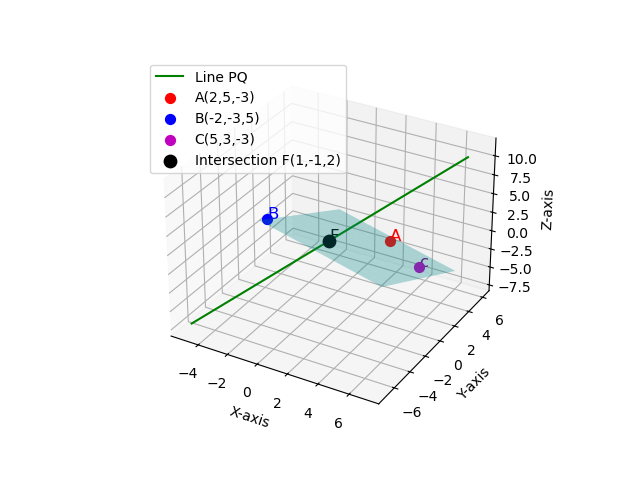
\includegraphics[height=0.5\textheight, keepaspectratio]{figs/figure1.png}
    \label{figure_1}
\end{figure}

\end{document}